\chapter{3D Vision}

Computer vision deals with:acquiring,processing,analyzing,and understanding,(might also include) 
generating or imagining visual data.

联系深度图,RGB图和点云的概念------ camera.RGB可以视作光打到深度图上,对RGB进行采样得到.

如何设计camera?多个光源照在一点,会产生blurring.因此产生了Pinhole camera.我们可以简单地描述其几何关系:
\begin{figure}[htbp]
	\centering
	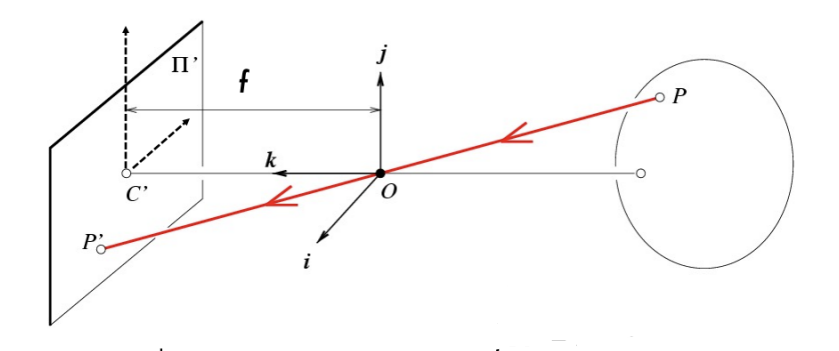
\includegraphics[scale=0.65]{figures/pinholecamera.png}
	\caption{pinhole camera的几何关系}
\end{figure}

满足如下变换
\begin{equation}
	\begin{cases}
		x^\prime &= f\disp\frac{x}{z}
		\\
		y^\prime &= f\disp\frac{y}{z}
	\end{cases}
\end{equation}

aperture size 实际上控制模糊程度和亮度.所以我们可以添加透镜 (lens),透镜可能产生畸变,因此真实相机往往复杂得多.

\section{Intrinsics}

上述变换的本质是一个映射$E: \mathbb{R}^3 \to \mathbb R^2$.投影操作,projection mapping.我们还需要完成两件事:
从实际的度量 (米)转换到pixel为单位,以及在图片中,左下角为零点,而非中心,因此需要添加offset.

\begin{equation}
	P=(x, y, z) \rightarrow P^{\prime}=\left(\alpha \frac{x}{z}+c_{x}, \beta \frac{y}{z}+c_{y}\right)
\end{equation}

能否用矩阵表示?很遗憾,这不是线性变换.因此引入homogeneous coordinate system,即增加一个维度作为除法.

\begin{equation}
	P_{h}^{\prime}=\left[\begin{array}{c}
		\alpha x+c_{x} z \\
		\beta y+c_{y} z \\
		z
	\end{array}\right]=\left[\begin{array}{cccc}
		\alpha & 0 & c_{x} & 0 \\
		0 & \beta & c_{y} & 0 \\
		0 & 0 & 1 & 0
	\end{array}\right]\left[\begin{array}{l}
		x \\
		y \\
		z \\
		1
	\end{array}\right]
\end{equation}

如果考虑相机坐标的screw,如下图,则需要进行简单的变换:
\begin{equation}
	\begin{cases}
		x &= \alpha(\hat x - \cot \theta \hat y) + c_x
		\\
		y &= \beta \disp\frac{\hat{y}}{\sin \theta} + c_y
	\end{cases}
\end{equation}

\begin{figure}[htbp]
	\centering
	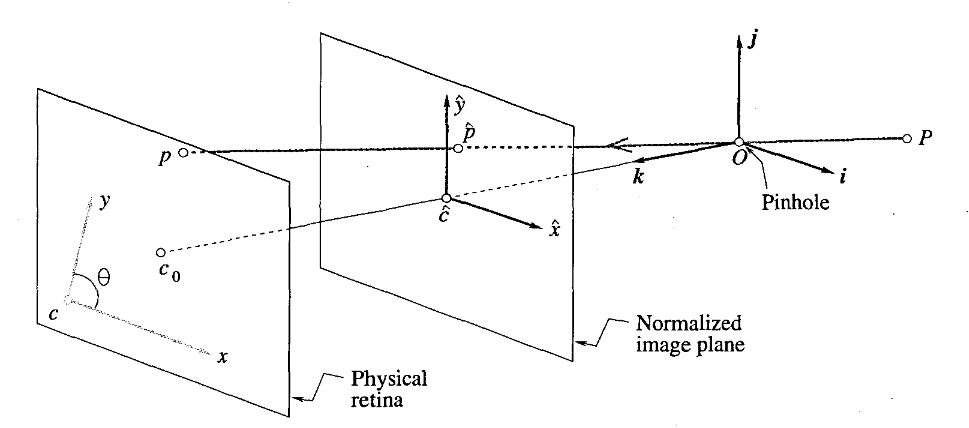
\includegraphics[scale=0.65]{figures/image_plane.png}
	\caption{成像过程坐标示意图}
\end{figure}

最后得到

\begin{equation}
	P^{\prime}=\left[\begin{array}{cccc}
		\alpha & -\alpha \cot \theta & c_{x} & 0 \\
		0 & \frac{\beta}{\sin \theta} & c_{y} & 0 \\
		0 & 0 & 1 & 0
	\end{array}\right]\left[\begin{array}{l}
		x \\
		y \\
		z \\
		1
	\end{array}\right]
\end{equation}

进行分解后表示为
\begin{equation}
	P^\prime = \bd M P = \bd K \begin{bmatrix}
		\bd I & \bd 0
	\end{bmatrix} P
\end{equation}

其中,矩阵$\bd K$定义为
\begin{equation}
	\bd K = \begin{bmatrix}
		\alpha & -\alpha \cot \theta & c_x
		\\
		0 & \frac{\beta}{\sin \theta} & c_y
		\\
		0 & 0 & 1
	\end{bmatrix}
\end{equation}

它是相机的内部参数,拥有$\alpha, \beta, \theta, c_x, c_y$五个自由度.

\section{Extinsics}
上一节当中,我们从camera coordina system->retina plane metric->image coordinate system.
但是我们希望完成从world coordinate到image coordinate system的转变.不难看出,
这是两个空间直角坐标系的平移和旋转变换.首先我们来看平移:

对于点$P$,如果要将其平移向量$\bm T$,则可以用如下的矩阵乘法表示:
\begin{equation}
	P^{\prime} \rightarrow\left[\begin{array}{ll}
		\mathbf{I} & \bm T \\
		\bm 0^\top & 1
	\end{array}\right]_{4 \times 4}\left[\begin{array}{c}
		x \\
		y \\
		z \\
		1
	\end{array}\right]
\end{equation}

对于旋转,我们先考虑平面直角坐标系的情形.假如最开始的坐标系为$S$,而$S^\prime$是将$S$逆时针旋转$\theta$,
那么可以得出如果要将$S$中的向量逆时针旋转$\theta$就是将坐标乘以$R_\theta$,其中
\begin{equation}
	R_{\theta} = \begin{bmatrix}
		\cos \theta & - \sin \theta
		\\
		\sin\theta & \cos \theta
	\end{bmatrix}
\end{equation}

原理即是将所有基底旋转$\theta$,坐标表示不变,则自然就随基底旋转.同样对于两个坐标系,$O\bm i \bm j \bm k$
和$O \bm i^\prime \bm j^\prime \bm k^\prime$,将前者坐标下的点$(x, y, z)$的基底向后者旋转,则需要左乘

\begin{equation}
	\bd R = \begin{bmatrix}
		\bm i^\prime \cdot \bm i  & \bm j^\prime \cdot \bm i & \bm k^\prime \cdot \bm i
		\\
		\bm i^\prime \cdot \bm j  & \bm j^\prime \cdot \bm j & \bm k^\prime \cdot \bm j
		\\
		\bm i^\prime \cdot \bm k  & \bm j^\prime \cdot \bm k & \bm k^\prime \cdot \bm k
	\end{bmatrix}
\end{equation}

但是,如果我们想在后者的坐标系中表示同一个向量(注意这两者的区别),那就需要左乘此矩阵的逆.由于此矩阵正交,所以也就是左乘其转置.

可以结合二维情形验证上述表达式.除此之外,我们还可以将旋转分解为三个方向的旋转:

\begin{equation}
	\begin{aligned}
		R_{x}(\alpha) &=\left[\begin{array}{ccc}
			1 & 0 & 0 \\
			0 & \cos \alpha & -\sin \alpha \\
			0 & \sin \alpha & \cos \alpha
		\end{array}\right],
		R_{y}(\beta) =\left[\begin{array}{ccc}
			\cos \beta & 0 & \sin \beta \\
			0 & 1 & 0 \\
			-\sin \beta & 0 & \cos \beta
		\end{array}\right],
		R_{z}(\gamma)= {\left[\begin{array}{lll}
				\cos \gamma & -\sin \gamma & 0 \\
				\sin \gamma & \cos \gamma & 0 \\
				0 & 0 & 1
			\end{array}\right] }
	\end{aligned}
\end{equation}

\begin{equation}
	P^{\prime} \rightarrow\left[\begin{array}{ll}
		\bd R & \bd 0 \\
		\bd 0^\top & 1
	\end{array}\right]_{4 \times 4}\left[\begin{array}{c}
		x \\
		y \\
		z \\
		1
	\end{array}\right]
\end{equation}

将平移和旋转结合,我们就有了统一的形式:

\begin{equation}
	P^{\prime}=K\left[\begin{array}{ll}
		I & 0
	\end{array}\right] P=K\left[\begin{array}{ll}
		I & 0
	\end{array}\right]\left[\begin{array}{ll}
		R & T \\
		0 & 1
	\end{array}\right]_{4 \times 4} P_{w}=K\left[\begin{array}{ll}
		R & T
	\end{array}\right] P_{w}
\end{equation}

其过程示意图如下:

\begin{figure}[htbp]
	\centering
	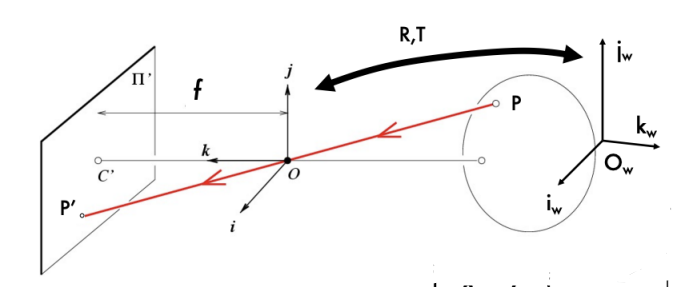
\includegraphics[scale=0.75]{figures/transform_all.png}
	\caption{坐标变换的全过程}
\end{figure}

若令$M = \bd K[\bd R \ \ \bd T]$,设其三个行向量为$\bm m_1, \bm m_2, \bm m_3$,则有
\begin{equation}
	P^\prime = \left(\frac{\bm{m}_{1} \bm P_{w}}{\bm{m}_{3} \bm P_{w}}, \frac{\bm{m}_{2} \bm P_{w}}{\bm{m}_{3} \bm P_{w}}\right)
\end{equation}

投影变换的性质:点映射成点,线映射成线,近大远小.

\section{weak perspective}

在弱透视模型中,点首先用正交投影投影到参考平面,然后用射影变换投影到图像平面.如下图:

\begin{figure}[htbp]
	\centering
	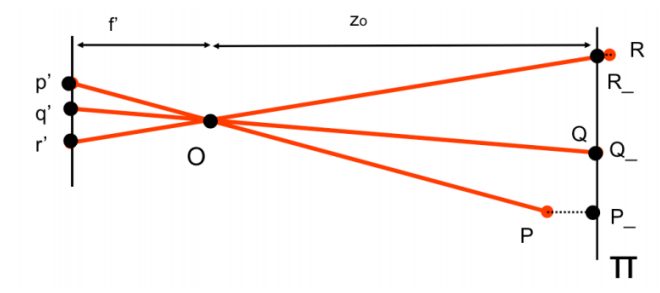
\includegraphics[scale=0.8]{figures/weak_perspective.png}
	\caption{weak perspective}
\end{figure}

这里的正交投影可以表示为

\begin{equation}
	\bd O = \begin{bmatrix}
		1 & 0 & 0 & 0
		\\
		0 & 1 & 0 & 0
		\\
		0 & 0 & 0 & z_0
		\\
		0 & 0 & 0 & 1
	\end{bmatrix} \xlongequal{\text{def}} 
	\begin{bmatrix}
		\bd O^\prime & \bm z_0
		\\
		\bm 0^\top & 1
	\end{bmatrix}
\end{equation}
即将所有$z$分量变为$z_0$.随后根据我们的变换公式
\begin{equation}
	\bm P^\prime = \bd K \begin{bmatrix}
		\bd I & \bm 0
	\end{bmatrix} \bd O 
	\begin{bmatrix}
		\bd R & \bd T
		\\
		\bm 0^\top & 1
	\end{bmatrix}
	\bm P
	= \bd K_{3\times 3} 
	\begin{bmatrix}
		\bd O^\prime \bd R & \bd O^\prime \bd T + \bm z_0
	\end{bmatrix}_{3\times 4} 
	\bm P_{4\times 1} 
\end{equation}

进一步,由于$\bd O^\prime$的第三行全零,因此中间矩阵的第三行是$[0, 0, 0, z_0]$.
记$\bd R_2, \bm t_2$分别是$\bd R, \bd T$的前两行,上式可以改写为

\begin{equation}
	\bm P^\prime = \bd K 
	\begin{bmatrix}
		\bd R_2 & \bm t_2
		\\
		\bm 0^\top & z_0
	\end{bmatrix}
	\bm P
\end{equation}

我们记
\begin{equation}
	\bd K = 
	\begin{bmatrix}
		\bd K_2 & \bm p_0
		\\
		\bm 0^\top & 1
	\end{bmatrix}, \quad 
	\bd K_2 = 
	\begin{bmatrix}
		\alpha & -\alpha \cot \theta
		\\
		0 & \frac{\beta}{\sin \theta}
	\end{bmatrix}, \quad
	\bm p_0 = 
	\begin{bmatrix}
		c_x 
		\\
		c_y
	\end{bmatrix}
\end{equation}

随后得到
\begin{equation}
	\bm P^\prime = 
	\begin{bmatrix}
		\bd K_2 \bd R_2 & \bd K_2 \bm t_2 + z_0 \bm p_0
		\\
		\bm 0^\top & z_0
	\end{bmatrix}
	\begin{bmatrix}
		x_w
		\\
		y_w 
		\\
		z_w
		\\
		1
	\end{bmatrix}
\end{equation}

不难看出,$\bm P^\prime$的第三个坐标 (即齐次项)为常数$z_0$,可以直接写成更简单的二维坐标形式:

\begin{equation}
	\bm p = \bd M \bm P
	\begin{bmatrix}
		\bd A & \bm b
	\end{bmatrix} \bm P
\end{equation}
其中
\begin{equation}
	\bd A = \frac{1}{z_0} \bd K_2 \bd R_2, \quad \bm b = \frac{1}{z_0} \bd K_2 \bm t_2 + \bm p_0
\end{equation}


更简单:orthographic (Affine) projection.正交投影.没有近大远小.这种投影在你不希望有近大远小的时候可以用到.